\documentclass[12pt, a4paper]{article}

\usepackage[a4paper, top=2.5cm, bottom=2.5cm, left=2.0cm, right=2.0cm, headheight=15pt]{geometry}
\usepackage[T1]{fontenc}
\usepackage[utf8]{inputenc}
\usepackage[english]{babel}
\usepackage{mathptmx}
\usepackage{enumitem}
\usepackage{microtype}
\nonstopmode
\setlist[itemize]{label=\textendash}

\usepackage[dvipsnames]{xcolor}
\definecolor{journalblue}{RGB}{26, 82, 118}
\definecolor{accentred}{RGB}{192, 57, 43}
\definecolor{tableheader}{RGB}{240, 244, 248}

\usepackage{graphicx}
\graphicspath{{../assets/}{assets/}{templates/assets/}{../../templates/assets/}{./}}

\usepackage{tikz}
\usetikzlibrary{shapes.geometric, arrows.meta, positioning, calc}

\usepackage{hyperref}
\hypersetup{
    colorlinks=true,
    linkcolor=journalblue,
    citecolor=journalblue,
    urlcolor=journalblue,
    pdftitle={Biophysical Kinetics and Ecological Systems Modeling}
}

\usepackage{amsmath, amssymb, amsfonts}
\usepackage{booktabs}
\usepackage{colortbl}
\usepackage{float}
\usepackage{setspace}
\onehalfspacing

\usepackage[font=small, labelfont=bf, labelsep=period]{caption}
\usepackage{parskip}
\usepackage{fancyhdr}
\pagestyle{fancy}
\fancyhf{}
\fancyhead[L]{\textcolor{journalblue}{\slshape\leftmark}}
\fancyhead[R]{\thepage}
\renewcommand{\headrulewidth}{0.4pt}

\usepackage{listings}
\usepackage[most]{tcolorbox}

\definecolor{codebeige}{RGB}{248, 249, 250}
\lstdefinestyle{academicstyle}{
    backgroundcolor=\color{codebeige},   
    commentstyle=\color{gray}\itshape,
    keywordstyle=\color{journalblue}\bfseries,
    basicstyle=\ttfamily\footnotesize,
    numbers=left, numberstyle=\tiny\color{gray},
    frame=none, breaklines=true
}
\lstset{style=academicstyle}

\newtcolorbox{biobox}[2][]{
    enhanced, colback=codebeige, colframe=journalblue!60,
    fonttitle=\bfseries\sffamily\small, coltitle=white, title={#2},
    arc=2pt, boxrule=0.6pt, top=4pt, bottom=4pt, left=6pt, right=6pt, #1
}

\newtcolorbox{theorybox}[2][]{
    enhanced, colframe=journalblue, boxrule=0pt, leftrule=3.5pt,
    colback=journalblue!5, arc=0pt, fonttitle=\bfseries\sffamily\small,
    coltitle=journalblue, title={#2}, top=5pt, bottom=5pt, left=8pt, right=8pt, #1
}

\usepackage[numbers,sort&compress]{natbib}

\begin{document}

\begin{titlepage}
    \begin{center}
        \vspace*{0.5cm}
        
\includegraphics[height=2.2cm]{university_seal.jpg}\par\vspace{0.4cm}
        {\scshape\Large Division of Biological Sciences \& Quantitative Ecology \par}
        \vspace{0.2cm}
        {\scshape\normalsize Biophysical Modeling and Systems Biology Group \par}
        \vspace{1.4cm}
        \rule{\linewidth}{1.2pt} \\[0.4cm]
        {\huge\bfseries Bio-Energetics, Trophic Dynamics, and Enzymatic Kinetics \par}
        \vspace{0.2cm}
        {\Large\itshape Mathematical Foundations of Thermodynamic Dissipation and Allosteric Saturation \par}
        \rule{\linewidth}{1.2pt} \\[1.2cm]

        \begin{minipage}[t]{0.45\textwidth}
            \textbf{\textcolor{journalblue}{Lead Author:}} \\
            Dr.~Jordan Taylor \\
            \texttt{jordan.taylor@university.edu}
        \end{minipage}
        \hfill
        \begin{minipage}[t]{0.45\textwidth}
            \begin{flushright}
                \textbf{\textcolor{journalblue}{Curriculum Track:}} \\
                BIO 401: Quantitative Biophysics \\
                \textit{Academic Year 2025--2026}
            \end{flushright}
        \end{minipage}
        \vfill
        {\today \par}
    \end{center}
\end{titlepage}

\pagenumbering{roman}
\section*{Executive Summary}
This report formulates quantitative biophysical models for ecological trophic transfers, bio-energetic conservation laws, and allosteric enzyme kinetics. Using Lindeman's trophic efficiency formulation ($\lambda \approx 10\%$), we examine thermodynamic energy dissipation across multi-tiered food webs. Furthermore, cooperative biochemical kinetics are analyzed via Hill equations and Lotka-Volterra non-linear dynamical systems.

\vspace{0.6cm}
\tableofcontents
\newpage
\pagenumbering{arabic}

\section{Bio-Energetic Conservation and Trophic Efficiency}
Energy transfer across trophic levels obeys the First and Second Laws of Thermodynamics~\cite{lindeman1942trophic, begon2006ecology}. Incident solar radiation ($10^6\,\mathrm{J}$) is captured by primary producers through photosynthesis, yielding net primary production (NPP).

\begin{theorybox}{Lindeman's 10\% Trophic Transfer Principle}
    The efficiency of energy transfer $\lambda$ from trophic tier $n$ to tier $n+1$ satisfies~\cite{lindeman1942trophic, keener2009mathematical}:
    \begin{equation}
        E_{n+1} = \lambda \cdot E_n, \quad \text{where } \lambda \approx 0.10
    \end{equation}
    The remaining $90\%$ of assimilated biomass is dissipated as cellular respiration, metabolic heat, and non-assimilated waste.
\end{theorybox}

\begin{figure}[H]
    \centering
    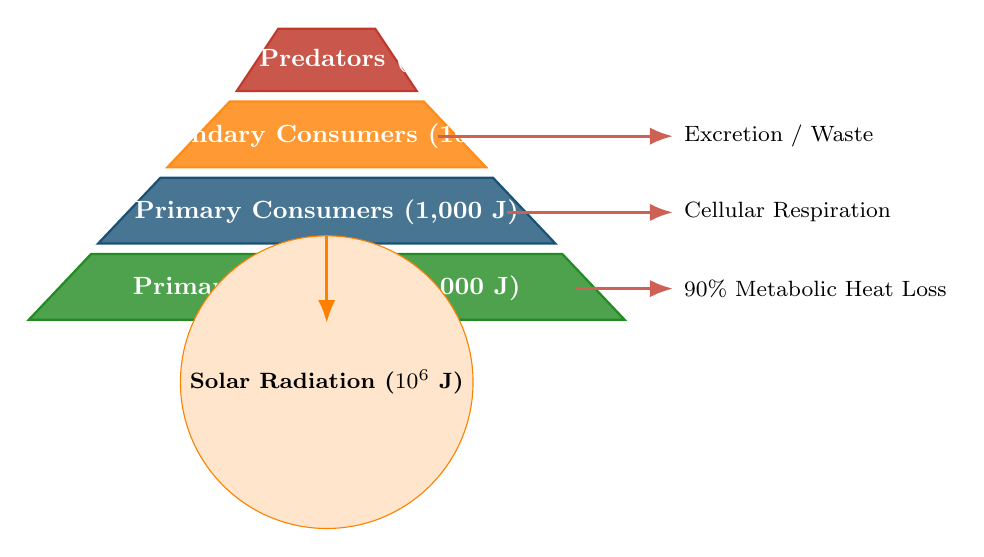
\begin{tikzpicture}[font=\sffamily, scale=0.88]
        \draw[fill=accentred!85, draw=accentred, thick] (-1.3, 3.3) -- (1.3, 3.3) -- (0.7, 4.2) -- (-0.7, 4.2) -- cycle;
        \node[text=white, font=\bfseries\small] at (0, 3.75) {Apex Predators (10 J)};
        
        \draw[fill=orange!80, draw=orange!90, thick] (-2.3, 2.2) -- (2.3, 2.2) -- (1.4, 3.15) -- (-1.4, 3.15) -- cycle;
        \node[text=white, font=\bfseries\small] at (0, 2.65) {Secondary Consumers (100 J)};
        
        \draw[fill=journalblue!80, draw=journalblue, thick] (-3.3, 1.1) -- (3.3, 1.1) -- (2.4, 2.05) -- (-2.4, 2.05) -- cycle;
        \node[text=white, font=\bfseries\small] at (0, 1.55) {Primary Consumers (1,000 J)};
        
        \draw[fill=ForestGreen!80, draw=ForestGreen, thick] (-4.3, 0.0) -- (4.3, 0.0) -- (3.4, 0.95) -- (-3.4, 0.95) -- cycle;
        \node[text=white, font=\bfseries\small] at (0, 0.45) {Primary Producers (10,000 J)};
        
        \draw[-Latex, very thick, draw=accentred!80] (3.6, 0.45) -- ++(1.4, 0) node[right, font=\footnotesize, text=black]{$90\%$ Metabolic Heat Loss};
        \draw[-Latex, very thick, draw=accentred!80] (2.6, 1.55) -- ++(2.4, 0) node[right, font=\footnotesize, text=black]{Cellular Respiration};
        \draw[-Latex, very thick, draw=accentred!80] (1.6, 2.65) -- ++(3.4, 0) node[right, font=\footnotesize, text=black]{Excretion / Waste};
        
        \node[circle, draw=orange, fill=orange!20, inner sep=3pt, font=\footnotesize\bfseries] (sun) at (0, -0.9) {Solar Radiation ($10^6$ J)};
        \draw[-Latex, very thick, draw=orange] (sun) -- (0, -0.05);
    \end{tikzpicture}
    \caption{Native TikZ schematic of the Ecological Trophic Energy Pyramid illustrating thermodynamic dissipation.}
    \label{fig:pyramid}
\end{figure}

\section{Allosteric Kinetics \& Population Dynamics}
Cooperative enzymatic saturation follows the Hill kinetic formulation:
\begin{equation}
    \label{eq:hill}
    v = \frac{V_{\max} [S]^h}{K_{0.5}^h + [S]^h}
\end{equation}
where $h$ denotes the Hill cooperativity coefficient ($h > 1$ represents positive cooperativity).

Table~\ref{tab:kinetics} summarizes experimental kinetic parameters across landmark enzyme systems.

\begin{table}[H]
    \centering
    \small
    \caption{Experimental catalytic constants and specificity metrics across enzyme classes.}
    \label{tab:kinetics}
    \begin{tabular}{@{} l c c c @{}}
        \toprule
        \rowcolor{tableheader}
        \textbf{Enzyme System} & \textbf{$K_m$ ($\mu\mathrm{M}$)} & \textbf{$k_{\mathrm{cat}}$ ($\mathrm{s}^{-1}$)} & \textbf{$k_{\mathrm{cat}}/K_m$ ($\mathrm{M}^{-1}\mathrm{s}^{-1}$)} \\
        \midrule
        Carbonic Anhydrase         & $12{,}000$ & $1{,}000{,}000$ & $8.3 \times 10^7$ \\
        Acetylcholinesterase       & $95$       & $14{,}000$      & $1.5 \times 10^8$ \\
        Triose Phosphate Isomerase & $470$      & $4{,}300$       & $9.1 \times 10^6$ \\
        Catalase                   & $25{,}000$ & $40{,}000{,}000$& $1.6 \times 10^9$ \\
        \bottomrule
    \end{tabular}
\end{table}

\section{Computational Dynamics}
Listing~\ref{lst:ode_sim} provides the Python routine for integrating non-linear Lotka-Volterra predator-prey dynamics.

\begin{biobox}[label={lst:ode_sim}]{Listing 1: Numerical Integration of Coupled Ecological ODEs}
\begin{lstlisting}[language=Python]
import numpy as np
from scipy.integrate import odeint

def lotka_volterra(state, t, r, a, b, m):
    N, P = state
    return [r * N - a * N * P, b * a * N * P - m * P]

t = np.linspace(0, 50, 1000)
sol = odeint(lotka_volterra, [40.0, 9.0], t, args=(0.5, 0.02, 0.1, 0.2))
\end{lstlisting}
\end{biobox}

\bibliographystyle{plainnat}
\bibliography{references}

\end{document}
